\documentclass[conference]{IEEEtran}
\usepackage{booktabs}
\usepackage{graphicx}
\usepackage{amsmath,amssymb}
\usepackage[T1]{fontenc}
\usepackage{microtype}
\usepackage[numbers]{natbib}
\usepackage[hidelinks]{hyperref}
\bibliographystyle{IEEEtran}
\graphicspath{{../figures/}}

% Shared macros. Names and numbers that appear more than once live here so that a
% value cannot drift between two mentions of it.

\newcommand{\pns}{prior-normalised skill}
\newcommand{\pss}{patient-specific skill}
\newcommand{\Pns}{Prior-normalised skill}
\newcommand{\Pss}{Patient-specific skill}

% The two objects previously both called "fitted template". Never write either
% phrase inline; renaming one edits these four lines and nothing else.
\newcommand{\maskref}{mask-fitted reference}        % fit to validation lesion masks; the content-free ceiling
\newcommand{\Maskref}{Mask-fitted reference}
\newcommand{\attden}{attention-fitted denominator}  % reference_baselines.fitted_template; fit to the arm's own attention
\newcommand{\Attden}{Attention-fitted denominator}

% Numbers quoted more than once, from the confirmatory artefacts.
\newcommand{\maskrefInplane}{0.8302}   % masks:inplane flat AUC
\newcommand{\maskrefSep}{0.8543}       % masks:separable flat AUC
\newcommand{\attdenMedian}{0.4208}     % median attention:inplane over the 40 H5 dumps
\newcommand{\probeDen}{0.8358}         % the probe's attention-fitted denominator
\newcommand{\centrePriorSlice}{0.6427} % model-free centre prior, slice AUC, \condA{}
\newcommand{\armSlot}{slot arm}

\newcommand{\preghash}{\texttt{4fd6e801157ecef5}}
\newcommand{\repourl}{https://github.com/BhaveshThapar/SlotMIL}

\newcommand{\armNG}{Normal Guidance}
\newcommand{\armGA}{gated ABMIL}
\newcommand{\condA}{\texttt{nodule\_present}}
\newcommand{\condB}{\texttt{malignancy}}
\newcommand{\condC}{\texttt{balanced\_presence}}
\newcommand{\condD}{\texttt{mosmed\_severity}}

% A verdict, typeset so a FAIL is never quieter than a PASS.
\newcommand{\PASS}{\textsc{pass}}
\newcommand{\FAIL}{\textbf{\textsc{fail}}}
\newcommand{\RPT}{\textsc{reported}}


\title{Position priors dominate instance-level localisation metrics for
weakly-supervised MIL in volumetric CT}

\author{\IEEEauthorblockN{Bhavesh Thapar}
\IEEEauthorblockA{University of Maryland, College Park\\
bthapar@terpmail.umd.edu}
\and
\IEEEauthorblockN{Mohammad Nayeem Teli}
\IEEEauthorblockA{University of Maryland, College Park\\
nayeem@umd.edu}}

\begin{document}
\maketitle

\begin{abstract}
Attention-based multiple-instance learning (MIL) is routinely credited with
localising findings in volumetric CT on the strength of instance-level AUC
against expert masks. We report a pre-registered ten-hypothesis evaluation of
what that number measures. On LIDC-IDRI, flat 3D instance AUC is within-slice
AUC in disguise: no scored arm separates the two by more than $0.02$ except
the one that injects an explicit axial prior, and a content-free reference fit
to lesion masks alone reaches $\maskrefSep$, above every trained arm. Explicit
prior injection is the single intervention that moves the measurement
($+0.1509$ patient-specific skill), and our instrument adjudicates that fix
rather than competing with it. Restricted to a lung segmentation the position
prior vanishes: the pre-registered template scores $0.4884$ inside the lung.
Which axis carries the prior is a property of the dataset --- on MosMed the
axial axis dominates ($0.8455$) exactly where LIDC's is empty. We recommend a
one-line convention any paper can adopt: report raw and in-organ instance AUC
side by side, and read the gap as that dataset's positional confound.
\end{abstract}

\begin{IEEEkeywords}
multiple-instance learning, weakly-supervised localisation, computed
tomography, evaluation methodology, pre-registration
\end{IEEEkeywords}

\section{Introduction}

Weakly-supervised MIL is trained on a bag-level label and asked, at evaluation
time, to say \emph{where} the finding is. The standard evidence is an
instance-level AUC: score every instance by its attention weight, label
instances by intersection with an expert mask, and pool. On volumetric CT the
instances are patch tokens over a stack of slices, and the number is reported
as three-dimensional localisation. That attention may do less work than
assumed is already visible at the classification level, where mean pooling
matches attention MIL across seven 3D tasks~\citep{harvey2026benchmark}; we
ask the corresponding question of the localisation number, and answer with
three claims.

\textbf{(i) The reported 3D metric is largely in-plane anatomical position.}
Flat instance AUC over a whole volume is statistically indistinguishable from
within-slice AUC for seven of eight scored arms. A content-free reference that
reads no image at all --- a $256$-number in-plane template fit to validation
\emph{lesion masks}, the \maskref{} --- scores above every trained arm, and an
untrained network reaches $0.7666$ at the $95$th percentile.

\textbf{(ii) The one intervention that adds real localisation is explicit
prior injection, and two tests that were not designed to agree both find it.}
Harvey-style \armNG{}~\citep{harvey2026normal} adds a KL term pulling the
attention's slice marginal towards a moment-matched Normal, and is both the
only arm whose \pss{} passes its falsifier and the only arm the axis gate
flags. The critique fails for that arm; our instrument validates their fix
against a stronger reference than the one they used.

\textbf{(iii) Which axis carries the prior is a property of the dataset.} We
pre-registered a stereotypy prediction and the data reversed it with power to
spare: COVID ground-glass is \emph{more} positionally stereotyped than a lung
nodule, on the axis LIDC leaves empty (Fig.~\ref{fig:contrast}).

\section{Setup and estimands}

\textbf{Data.} LIDC-IDRI~\citep{armato2011lidc}: $999$ series over $991$
patients, split $700/149/150$ by patient at seed $2027$, a split the protocol
was never developed against. Frozen DINOv2 ViT-B/14
features~\citep{oquab2024dinov2}, $16{\times}16$ patches per slice; instance
labels from four-radiologist consensus masks rasterised to the grid.
MosMed~\citep{morozov2020mosmed} enters for one hypothesis only ($50$ of
$1110$ studies carry masks). Four conditions are declared; \condA{} carries
the hypothesis family, and ``all three conditions'' below means the three LIDC
conditions (companion, \S3).

\textbf{Arms.} Ten: mean pooling, ABMIL~\citep{ilse2018}, gated ABMIL,
multi-head ABMIL, CLAM-SB~\citep{lu2021clam}, DSMIL~\citep{li2021dsmil},
TransMIL~\citep{shao2021transmil}, slot attention~\citep{locatello2020slot}
with a diversity term, a fixed centre Gaussian, and
\armNG{}~\citep{harvey2026normal}; five seeds each; eight are scored. Every
AUC is a patient-clustered bootstrap over per-bag AUCs, $10{,}000$ replicates.

\textbf{Two templates, two names.} Two objects here are each an in-plane
template fit on validation. The \emph{\maskref{}} is fit to \emph{lesion
masks}: it reads no image or attention and sets the content-free ceiling
($\maskrefInplane$ in-plane, $\maskrefSep$ separable). The \emph{\attden{}}
is the same rule fit to \emph{the arm's own attention}: it is the
pre-registered reference $A_t$ of \pns{} $= (A-A_t)/(1-A_t)$, and its median
over the scored dumps is $\attdenMedian$. The first is an oracle no arm
reaches; the second adapts to the arm being scored. \Pss{} is
$A_{\text{real}} - A_{\text{cross-patient}}$: the score that survives
swapping whose masks the attention is scored
against~\citep{borji2013,bylinskii2019}.

\begin{figure*}[t]
\centering
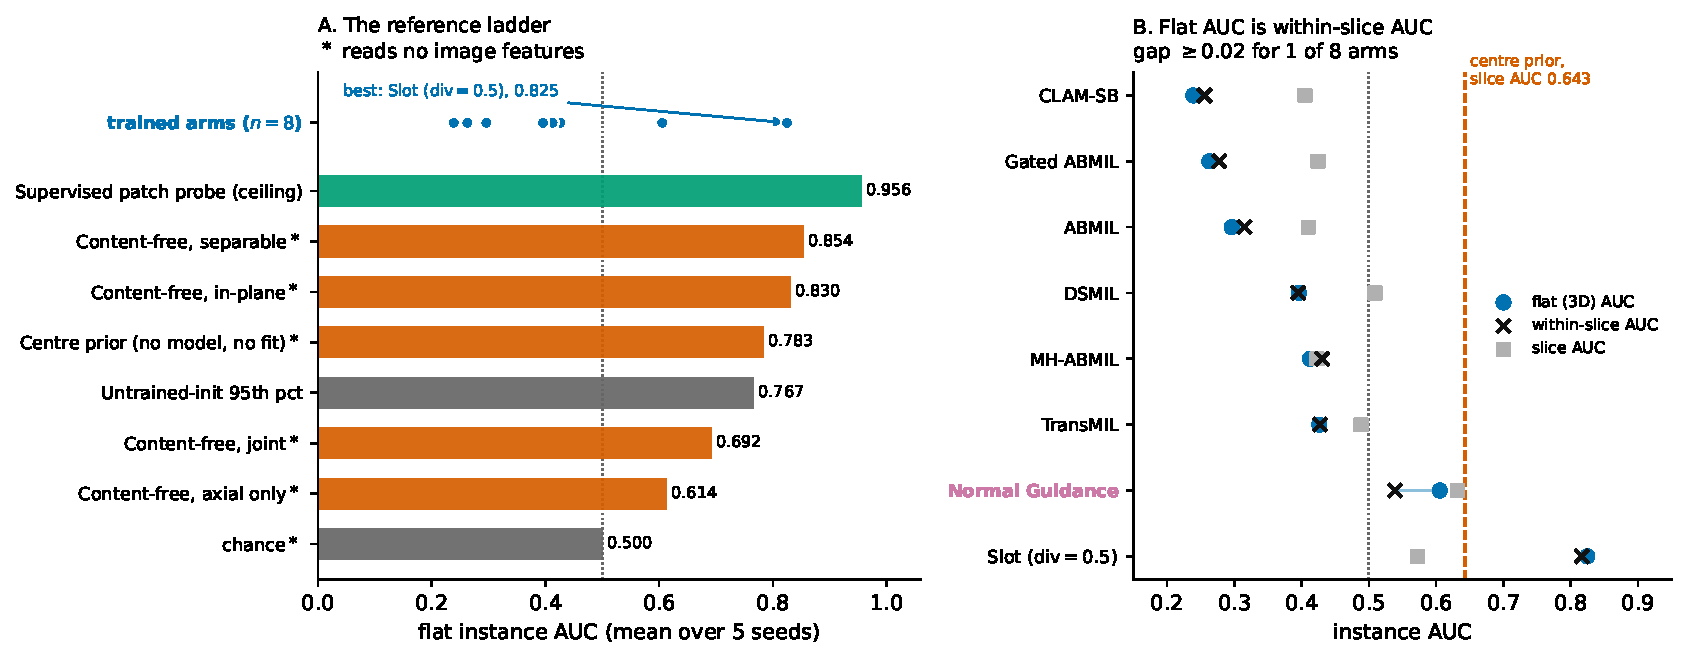
\includegraphics[width=\textwidth]{fig1_reference_ladder.pdf}
\caption{\textbf{Left:} the reference ladder on \condA{}. Starred references
are \maskref{}s: they read no image features and are computed from lesion
masks and patch geometry. The best trained arm --- the \armSlot{}, $0.8247$
--- sits below the separable \maskref{} and barely above an untrained
network's $95$th percentile. \textbf{Right:} flat, within-slice and slice AUC
per arm; flat and within-slice coincide for every arm but \armNG{}, and no
arm's slice AUC exceeds the model-free centre prior.}
\label{fig:ladder}
\end{figure*}

\section{Results}

\subsection{The floor, the ceiling, and the axis (H1--H3)}

$|\text{flat} - \text{within-slice}|$ exceeds $0.02$ for one of eight arms
(the falsifier required a majority); the positive controls separate
(\texttt{masks:axial} $0.1064$, centre prior $0.0518$), so the test can
detect axial content when present. The one arm over the bar is \armNG{}
($0.0669$, next-highest $0.0190$). No trained arm reaches the centre prior's
slice AUC of $\centrePriorSlice$; the best, \armNG{} at $0.6318$, is a
statistical tie (paired per-bag $\Delta$, patient-clustered over five seeds:
$+0.0109$ $[-0.0078, +0.0300]$), and every other arm's interval sits entirely
on the prior's side. The $95$th-percentile instance AUC over $30$ untrained
initialisations is $0.7666$ against a bar of $0.70$: chance is not the floor,
and a reported $0.79$--$0.82$ is inside or barely above the untrained range.

\subsection{What survives normalisation (H4, H5)}

Median \pss{} is $-0.0466$ and five of eight arms are negative: scoring an
arm's attention against \emph{another patient's} masks beats scoring it
against the right ones. No arm's \pns{} exceeds $0.30$ (max $+0.1990$); one
seed sits at $0.3432$ and is reported rather than absorbed, because the unit
was declared before that seed existed. Because the declared \attden{} sits
below chance for $24$ of $40$ dumps --- which makes a stay-below-the-bar
hypothesis easier to pass --- the companion recomputes the identical statistic
with the denominator floored at $0.5$: no verdict moves, and flooring lowers
the maximum wherever it binds.

\subsection{Prior injection is the exception (H6)}

The falsifier stated that if \pss{} rises by $\geq 0.02$ under prior
injection, the critique fails for that arm. It rose $+0.1509$, from $-0.1019$
to $+0.0490$; we report the failure. Three things make it the second finding.
Magnitude: \armNG{} is one of only three arms with positive \pss{} at all,
and the only one that also clears the axis gate. Independence: the axis gate
and the skill are different statistics on different artefacts, and both
single out the same arm of eight. Mechanism: the arm's only departure from
its base is a KL term naming the axial coordinate, so the gain cannot be
attributed to a stronger backbone. Nothing in the architecture sweep adds
localisation; a loss term that names the axis explicitly does --- yet its
slice AUC still only ties the centre prior, so prior injection moves the
measurement without solving the problem.

\subsection{The power gate, and its scope (H7)}

The constructive half is gated: a supervised patch probe must clear $0.50$
\pns{} while every content-free baseline stays below $0.05$. The gate passes
on \condA{} ($0.7305$; content-free members $\leq 0.0105$) and \condB{}
($0.7036$), and fails on \condC{} ($0.4772$): \textbf{we recommend the
estimands only where the per-condition gate passes.} The gate's stochastic
members were originally computed from a single shared realisation, under
which H7 \emph{failed}; the amendment replicating them ($30$ draws, mean over
draws, the stricter aggregation left in force) was committed before the
replicated numbers existed, and the full measurement history is in the
companion.

\subsection{The portable convention (H8)}

H8 was declared two-sided, with it written in advance that if restricting to
lung removed the prior, that becomes the recommendation rather than a defeat.
It does: the lung is $25.2\%$ of a bag, and inside it the pre-registered
\attden{} scores $0.4884$ against a bar of $0.65$ (set against the
unrestricted template's $0.786$ on discovery), all three LIDC conditions
agreeing. No arm's \attden{} beats chance inside the lung. Applied to the
arms' own attention --- Recommendation~1 on ourselves --- the same
restriction confirms the reading (companion): the strongest trained arm, the
\armSlot{} at flat $0.8247$, falls to $0.5560$ inside the lung --- far the
largest loss of the eight --- and is also the arm whose template loses the
most ($-0.300$) and the owner of H5's one over-bar seed. The
``interpretable'' arm looked best precisely because it learned lung geometry.

\begin{figure}[t]
\centering
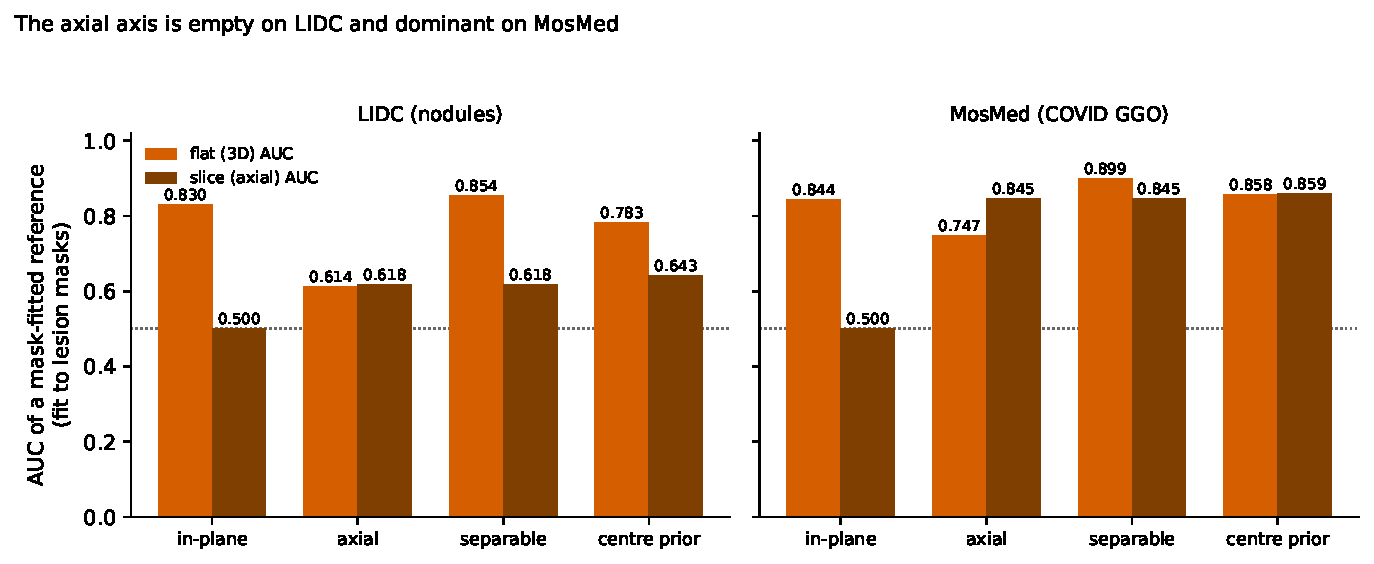
\includegraphics[width=\columnwidth]{fig4_dataset_contrast.pdf}
\caption{\Maskref{}s, LIDC versus MosMed. The axial axis is empty on LIDC and
dominant on MosMed; no training is involved in any bar.}
\label{fig:contrast}
\end{figure}

\subsection{The dataset contrast (H9)}

H9 predicted prior dominance would track positional stereotypy with the lung
nodule as the more stereotyped finding; it was reversed with power to spare
(median observed separation $-0.2495$ against a required $+0.0560$). COVID
ground-glass is peripheral in-plane and basal axially, and MosMed's
mask-fitted axial template reaches slice AUC $0.8455$ against LIDC's
$0.6180$. Which axis carries the prior must be measured on the cohort being
reported, and Fig.~\ref{fig:contrast} costs no training to produce.

\section{Recommendations}

\begin{enumerate}\itemsep1pt
\item \textbf{Report raw and in-organ instance AUC side by side}; the gap is
that dataset's positional confound. One segmentation, no retraining.
\item \textbf{Report the axis decomposition} (flat, within-slice, slice). If
flat equals within-slice, the metric is not measuring the third dimension.
\item \textbf{Measure the floor}: a content-free positional reference and an
untrained-initialisation percentile. Chance is not the floor.
\item \textbf{Normalise against the \attden{} and gate it} on the
per-condition supervised-probe test; where the gate fails, fall back to 1.
\end{enumerate}

\section{Pre-registration}

Every threshold, arm and estimand was frozen in a machine-readable
pre-registration (hash \preghash{}) before any confirmatory number existed;
analysis code reads parameters only from that file and raises on anything
undeclared. The full falsifier table, verdicts across conditions, the dated
amendment chain, the multiplicity analysis, and the declared-versus-reported
diff are in the companion and at \url{\repourl}.

\bibliography{../refs}
\end{document}
